%% ------------------------------------------------------------------------- %%
\chapter{Trabalhos relacionados}
\label{cap:trabalhos-relacionados}



%% ------------------------------------------------------------------------- %%
\section{Recuperação de trecho de código-fonte ou \textit{Code retrieval}}
\label{sec:code-retrieval}

\subsection{Definição}\label{sec:code-retrieval-definicao}
De acordo com \cite{Chen-bi-variational-autoencoder:2018}, a tarefa do \textit{code retrieval} consiste em:

\emph{Dado uma descrição em linguagem natural, recuperar o trecho de código-fonte mais relevante, tal que os desenvolvedores possam encontrar rapidamente os trechos de código que atendam as suas necessidades.}

Para \cite{cambronero-deep-learning-code-search:2019}, o objetivo do \textit{code search} é recuperar um trecho de código-fonte a partir de um enorme repositório de código-fonte, que mais se aproxima da intenção do desenvolvedor, expressa em linguagem natural. 

Adotaremos a mesma definição proposta por \cite{iyer-etal-2016-summarizing, Yao-coacor:2019} para \textit{code retrieval}:

Dado uma questão em linguagem natural $Q$ e um conjunto com os trechos de código-fonte candidatos $\mathbb{C}$, \textit{code retrieval} recupera o trecho de código $C^{*} \in \mathbb{C}$ que corresponde a dada questão.

Formalmente, para um conjunto de treinamento com pares de questões e trechos de código-fonte (<questão, trecho de código-fonte>), e.g., dados coletados do StackOverFlow por \cite{yao-2018}, \textit{code retrieval} é definido como:

\textbf{Code Retrieval}: Dada uma questão em linguagem natural $Q$, um modelo $F_{r}$ irá aprender a recuperar o trecho de código-fonte $C^{*} \in \mathbb{C}$ com a maior pontuação:

\begin{equation}\label{eq:code-retrieval}
C^{*} = \underset{C \in \mathbb{C}}{argmax}\text{ } F_{r}(Q , C)
\end{equation}

Neste trabalho, tanto o termo \textit{code retrieval} quanto \textit{code search} irão referir-se ao mesmo problema.



\section{Joint Embeddings}

Segundo \cite{Goodfellow-et-al-2016:representation-learning}, um fator importante a ser levado em consideração é a forma como os dados são representados. Uma boa representação consegue identificar as características relevantes e os fatores causadores dos dados observados. Estas características são invariantes em relação aos dados de entrada. Uma boa representação pode ser utilizada em outras tarefas, em diferentes modalidades, i.e., o modelo encontrado que é útil para um cojunto de dados que segue uma distribuição $P1$, pode ser útil para um conjunto de dados que segue uma distribuição $P2$. Desde que os fatores encontrados para $P1$, sejam relevantes ou expliquem parte da variação em $P2$.

No caso do código-fonte, ao tratá-lo como um texto formado por uma sequência de palavras, uma boa representação é um vetor de representação distribuída. As redes neurais generalizam bem quando as palavras são representadas através de vetores de representação distribuída em comparação a um \gls{one-hot-encoding}. Representação distribuída induz a um rico espaço de similaridade, no qual conceitos semanticamente similares (ou dados de entrada) estão próximos, uma propriedade que não está presente em representações puramente simbólicas \citep{Goodfellow-et-al-2016:representation-learning}.



\subsection{Token Embedding}

De acordo com \cite{cambronero-deep-learning-code-search:2019}, \textit{embedding} é uma forma de representar um dado de entrada através de um vetor com valores reais ($\mathbb{R}$). \textit{Embedding} pode ser definida como uma função $\mathbb{E}$, tal que:

\begin{equation}
    \mathbb{E}: \mathbb{X} \rightarrow \mathbb{R}^{d}
\end{equation}

A função $\mathbb{E}$ mapeia um dado de entrada $x$, $x \in \mathbb{X}$, para um vetor de \gls{representacao-distribuida} correspondente em um espaço vetorial de dimensão $d$. O vetor de representação distribuída utiliza a hipótese distribucional, no qual palavras de um mesmo contexto tem significados similares.

Uma opção para a função $\mathbb{E}$ é utilizar o algoritmo não-supervisionado \textit{word2vec}. O \textit{word2vec} utiliza o algoritmo \textit{skip-gram} ou \acrshort{cbow}. A diferença basicamente entre eles é que o \acrshort{cbow} prediz uma palavra de acordo com as palavras do contexto e o \textit{skip-gram} faz o inverso, prediz as palavras do contexto dado uma palavra alvo \citep{mikolov2013distributed}.

Por exemplo, dado o trecho de código-fonte abaixo:

\begin{mypython}{Python: Exemplo de código para escrever em um arquivo}
with open(filename, mode) as file:
    file.write(text)
\end{mypython}

Removendo os acentos, tabulações, quebra de linha e as pontuações, o código-fonte pode ser representado por um vetor formado pela seguinte sequência de palavras:

\begin{mypythonembedding}{Trecho de código-fonte representado através de vetor de \textit{tokens}.}
  ['with', 'open', 'filename', 'mode', 'as', 'file', 'file', 'write', 'text']
\end{mypythonembedding}

Neste caso, ao utilizar o \textit{skip-gram} do \textit{wordvec} para a palavra \emph{file}. Ele representará a palavra \emph{file} próxima das palavras \emph{mode}, \emph{as}, \emph{file}, \emph{write}, caso o parâmetro \textit{window} seja $2$. O parâmetro \textit{window} define basicamente quantas palavras a direita e a esquerda fazem parte do contexto.

\begin{mypythonembedding}{Palavra \textit{file}, em amarelo, e as palavras similares, em verde.}
  ['with', 'open', 'filename', |\colorbox{green}{mode}|, |\colorbox{green}{as}|, |\colorbox{yellow}{file}|, |\colorbox{green}{file}|, |\colorbox{green}{write}|, 'text']
\end{mypythonembedding}

\begin{figure}[h]
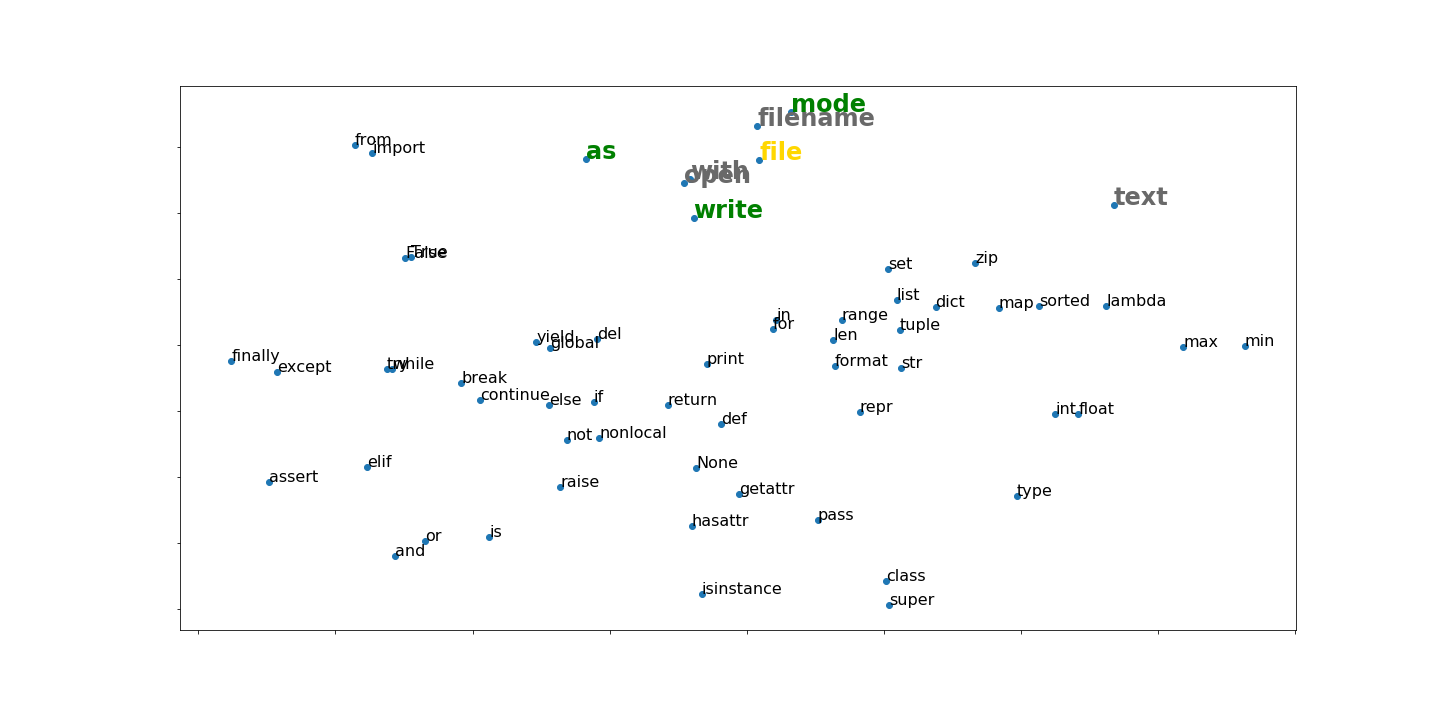
\includegraphics[width=1\textwidth]{figuras/cap-trabalhos-relacionados/code-tsne-output.png}
\caption{Total de perguntas sobre Python e SQL no \textit{StackOverFlow} até 20 de março de 2019. Google and the Google logo are registered trademarks of Google LLC, used with permission.}
\label{fig:bigquery-total-questions-python-sql-stackoverflow}
\end{figure}


\subsection{Bags and sequence embeddings}

Conforme \cite{cambronero-deep-learning-code-search:2019}, os vetores de representação distribuída de cada termo ou palavra, i.e., os \textit{tokens embeddings}, podem ser tratados como \textit{bags}. Neste caso, a ordem das palavras não importa.

\section{Trabalhos relacionados}\label{sec:code-retrieval-trabalhos-relacionados}

\textit{Code search} ou \textit{code retrieval} busca associar um texto em linguagem natural a um código-fonte. Esta associação tem diversas aplicações em engenharia de software conforme exposto no capítulo~\ref{cap:introducao}.

O trabalho de \cite{Allamanis-bimodal-source-code-natural-language:2015} foi um dos primeiros a abordar o problema do \textit{code retrieval}. Neste trabalho utilizou-se vetores de \gls{representacao-distribuida} tanto para as descrições quanto para os trechos de código-fonte. Uma função de classificação foi utilizada para combinar os vetores. A combinação foi feita usando operações aditivas ou multiplicativas. Ao final, o valor obtido a partir da função de classificação é convertida em probabilidade para avaliar qual trecho de código-fonte é mais relevante para uma determinada questão.

Já \cite{iyer-etal-2016-summarizing} utilizaram uma rede neural recorrente, mais especificamente \acrshort{lstm} com o \gls{mecanismo-atencao} para classificar o trecho de código-fonte de acordo com a questão. \cite{Chen-bi-variational-autoencoder:2018} utilizaram \acrfull{vae} para obter um vetor de \gls{representacao-distribuida} do código-fonte e descrição. E utilizaram algoritmos de similaridade para recuperar o trecho de código-fonte.

\cite{Gu-deep-code-search:2018} utilizaram o conceito de \textit{joint embedding}, uma técnica para juntar dados heterogêneos em um mesmo espaço vetorial tal que conceitos similares de categorias diferentes ocupem regiões próximas do espaço. Para mapear as questões e trechos de código-fonte para o mesmo espaço vetorial, \cite{Gu-deep-code-search:2018} utilizaram uma rede neural bi-\acrshort{lstm} com uma camada \textit{maxpool} ao final. Para verificar a similaridade entre os vetores, foi utilizado a função de similaridade \textit{cosine}.

\cite{Yao-coacor:2019} aprimoraram o \textit{code retrieval} combinando anotações com trechos de código-fonte. As anotações foram geradas por um modelo e aprimoradas através de aprendizagem por reforço (\textit{reinforcement learning}). Durante a aprendizagem por reforço, as anotações foram avaliadas para maximizar o sucesso na tarefa de \textit{code retrieval}.

Um grupo do Facebook\footnote{\url{https://www.facebook.com}}\citep{Sachdev-neural-code-search:2018} utilizou uma abordagem diferente. A hipótese inicial deles é que o código-fonte contém informações suficientes para ser utilizada no problema do \textit{code retrieval}. Diferente dos trabalhos citados anteriormente, eles não fizeram uso inicialmente das questões. Para cada método ou função de uma classe em um projeto de código-aberto, eles extraíram nome de método, chamadas de API, constantes e textos literais. A partir destas informações extraídas, eles criaram um vetor de representação distribuída para o método, combinando o vetor de representação distribuída com o peso \acrshort{tf-idf} de cada palavra. 

Inicialmente, o resultado obtido foi comparável a outros métodos largamente utilizados em recuperação de documentos (information retrieval). Verificou-se que os acertos ocorriam apenas quando as perguntas continham as mesmas palavras dos trechos de código-fonte. Para aprimorar, eles mapearam palavras presentes nas perguntas para palavras equivalentes no código-fonte. Isto foi feito através de um treinamento supervisionado. Após este mapeamento, eles conseguiram responder corretamente 2/3 dos pares de questões extraídos do StackOverFlow. Para eles, a resposta é considerada correta quando ela aparece entre os 10 primeiros resultados.